\documentclass[10pt,letterpaper]{book}
\usepackage[utf8]{inputenc}
\usepackage[spanish]{babel}
\usepackage{amsmath}
\usepackage{amsfonts}
\usepackage{amssymb}
\usepackage{graphicx}
\usepackage{empheq}
\usepackage{svg}
\usepackage{hyperref}
\usepackage{hypcap}
\usepackage[spanish,onelanguage,linesnumbered,ruled,vlined]{algorithm2e}
\usepackage{titling}
\pretitle{%
  \begin{flushright}
  \vspace{-9.5cm}
%  
\includegraphics[width=5cm,natwidth=472,natheight=531]{logo} \\[7cm]
  
\includegraphics[width=5cm]{logo} \\[6cm]
  \end{flushright}
  \begin{center}
  \LARGE
}
\posttitle{\end{center}}
\usepackage[left=4cm,right=2.5cm,top=3cm,bottom=4cm,includehead,includefoot,headheight=15pt]{geometry}
\usepackage{setspace}
\setstretch{0.4}
\usepackage{fancyhdr}
\date{27 de Noviembre 2018}
\fancyhf{}
\renewcommand{\headrulewidth}{0pt} % optional
%\fancyhead[L]{\nouppercase{\leftmark} \hfill Section \nouppercase{\rightmark}}
\fancyhead[L]{Introducción al Método de Steffensen}
\cfoot{\thepage}
\pagestyle{fancy}
\author{
Alejandra Gabriela Rossel Ríos\\
\texttt{Reg: 217045499}
\and
Leonardo H. Añez Vladimirovna\\
\texttt{Reg: 217002498}
\and
Pablo Michael Tardío Ventura\\
\texttt{Reg: 217064957}
\and
Javier Selaya Melgar\\
\texttt{Reg: 217048137}
\and
Liz Dara Choque Coca\\
\texttt{Reg: 217011810}
\and
Maikol Bryan Sanchez Castro\\
\texttt{Reg: 217064531}
\and
Cristian Terceros Coca\\
\texttt{Reg: 217050662}
}
\title{
Métodos Numéricos\\ ${ }$\\
\textbf{Una Introducción al Método de Steffensen}
\\ ${ }$\\
\small Facultad de Ingeniería en Ciencias de la Computación y Telecomunicaciones\\}

\begin{document}
\maketitle
\section*{Tabla de Contenidos}
\begin{itemize}
\item \textbf{Objetivos} 
\item \textbf{Introducción}
\item \textbf{Método del Punto Fijo}
\item \textbf{Método $\Delta^2$ de Aitken}
\item \textbf{Aplicando el Método de Steffensen}
\item \textbf{Conclusión}
\end{itemize}
\frontmatter
\section*{Objetivo}
En esta monografia queremos dar a conocer el Método de Steffensen para la resolucion de Ecuaciones, ademas de comprender como funciona el algoritmo de este método.
\section*{Introducción}
En análisis numérico, el Método de Steffensen es una técnica para hallar la raíz de una ecuación, similar al método de Newton, llamado así por Johan Frederik Steffensen. Este método también logra una convergencia cuadrática pero sin usar las derivadas como lo hace el método de Newton. Para ser mas precisos, el Método de Steffensen es una combinación del método del punto fijo y el método $\Delta^2$ de Aitken.
\subsubsection*{Johan Frederik Steffensen}
\textit{(28 de Febrero 1873 (Copenhagen) - 20 de Diciembre 1961)} Fue un Matemático Danes, estadísta y actuario que realizo investigaciones en los campos de calculo de diferencias infinitesimales e interpolación. Fue profesor de Ciencias Actuarias en la  Universidad de Copenhagen desde 1923 hasta 1943. Se le atribuyen principalmente la \textit{Desigualdad de Steffensen} y el \textit{Método de Steffensen.}
\section*{Método del Punto Fijo}
Es un método iterativo que permite resolver ecuaciones no necesariamente lineales. En particular se pueden utilizar para determinar raíces de una función de la forma $f(x)=0$ transformandola algebraicamente a la forma $x=g(x)$ y utilizando un punto $p_0$ como punto de partida.
\subsubsection{Teorema}
\begin{center}
\fbox{
\begin{minipage}{35em}
\textit{Sea $g\in [a,b]$ tal que $g(x)\in [a,b]$. Suponga ademas que $g'$ existe en $(a,b)$, (es decir es continua en ese intervalo) y que una constante $0<k<1$ existe con:
$$|g'(x)|\leq k \forall x \in (a,b)$$
Entonces, para cualquier numero $p_0$ en $[a,b]$ la secuencia 
$$p_n = g(p_{n-1})$$
converge a un unico punto $p$ en el intervalo.}
\end{minipage}}
\end{center}

\begin{algorithm}[H]
  Con: 
   $p_0$ \\
  \For{$i=0,1,\ldots$, hasta que se satisfaga}{
  \vspace{0.2cm}  
  Calcular: 
  \fbox{$p=g(p_0)$}\\
  \vspace{0.2cm} 
  
  \uIf{$|p-p_0|<Tolerancia$}{
   \vspace{0.2cm}
   Detener
   }
   \uElse{
   \vspace{0.2cm}
   $p_0=p$
  }
 }
 \caption{Método del Punto Fijo}
\end{algorithm}
\subsubsection*{Ejemplo}
Tenemos la siguiente función y queremos hallar su raíz:
	$$f(x)=sin^2(x)-x^2+1$$
Si realizamos la grafica utilizando $Geogebra$ tendremos la siguiente figura:
\begin{figure}[h]
\centering
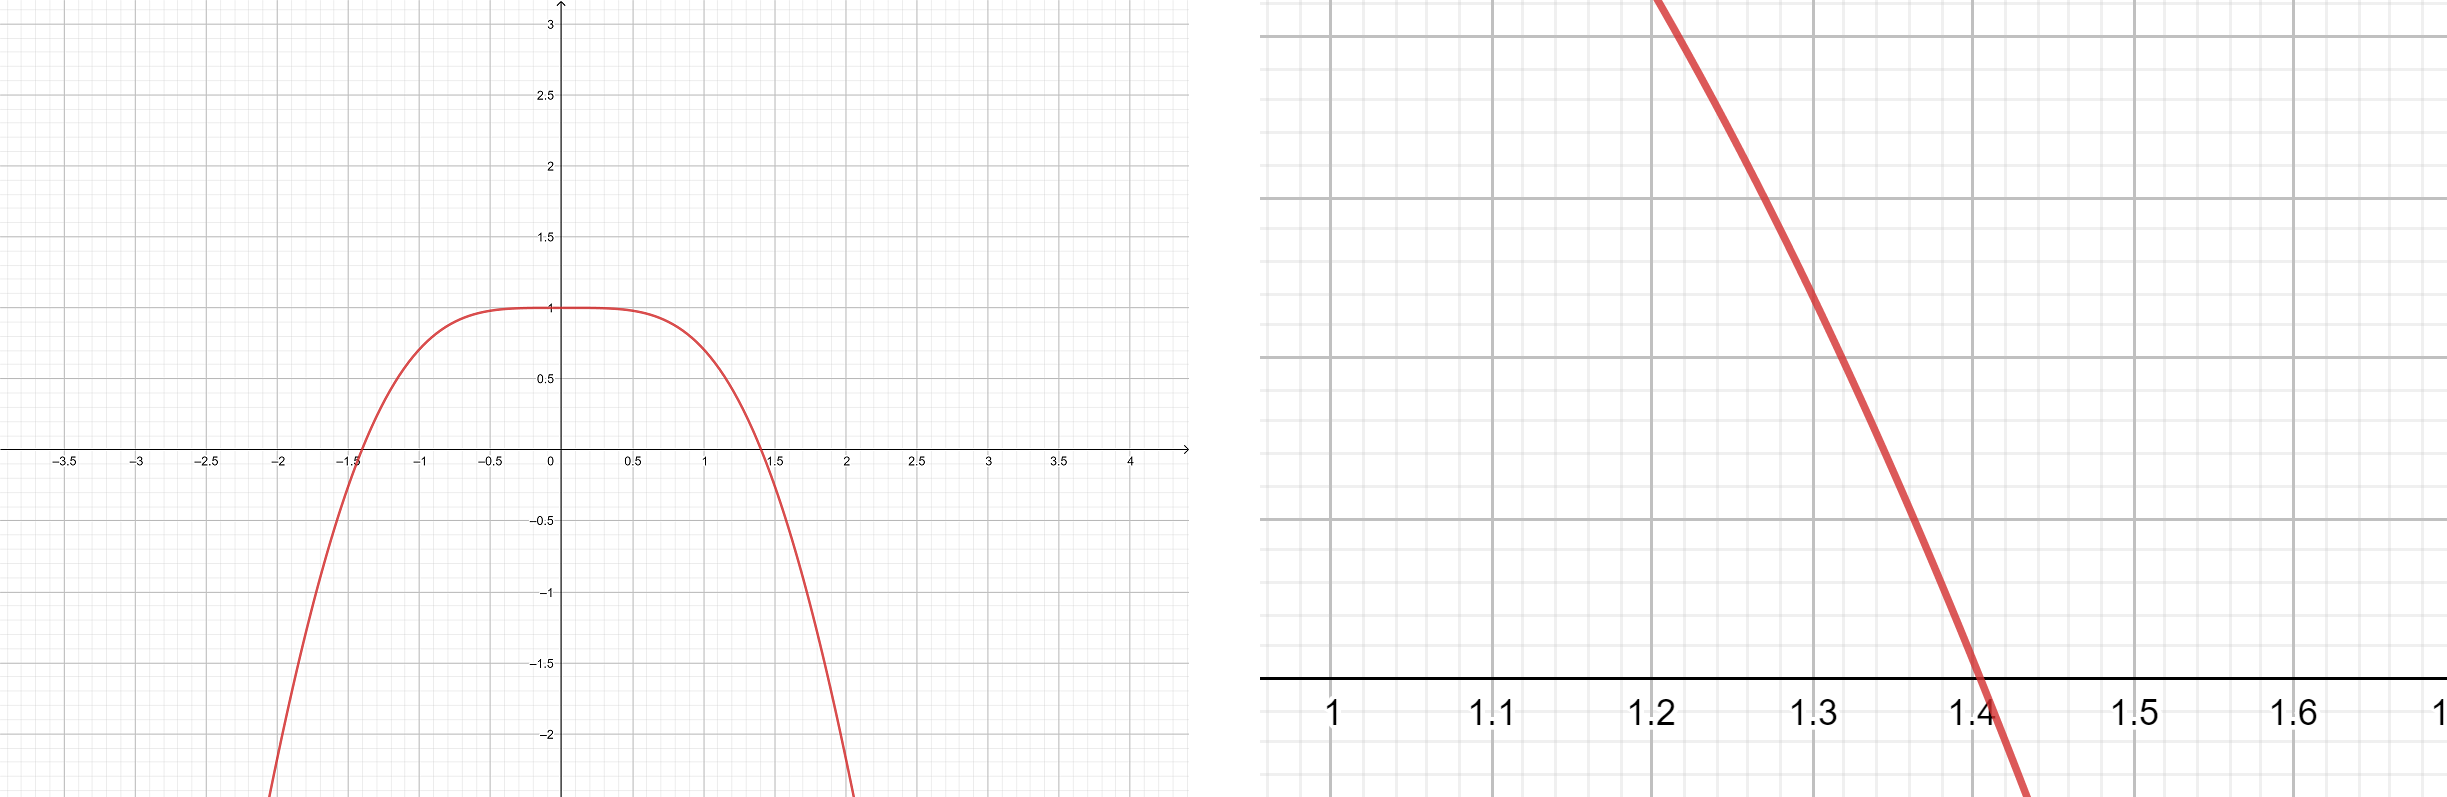
\includegraphics[width=12cm]{puntofijo1}
\caption{Grafica realizada en Geogebra, la grafica de la derecha es una parte con zoom de la función.}
\end{figure}
Si despejamos modificamos la funcion algebraicamente a la forma $x=g(x)$, tendremos: 
$$g(x)= \sqrt{sin^2(x)+1}$$
Con esto procedemos a realizar el metodo del punto fijo, como primera aproximacion tendremos $p_0=1$. 

\begin{itemize}
\item \textbf{Iteración:} 0
$$p_0=1 \hspace{1cm} g(p_0)=1.306932828523934$$
\item \textbf{Iteración:} 1
$$p_1=1.306932828523934 \hspace{1cm} g(p_1)=1.3899557402473888$$
\item \textbf{Iteración:} 2
$$p_2=1.3899557402473888 \hspace{1cm} g(p_2)=1.4027300644478016$$
\item \textbf{Iteración:} 3
$$p_3=1.4027300644478016 \hspace{1cm} g(p_3)=1.404285826470638$$
\end{itemize}

Realizando el algoritmo del Punto Fijo, obtenemos la siguiente tabla para una tolerancia de $0.0005$.
\begin{table}[h]
\centering
\begin{tabular}{|c|c|c|c|}
\hline
Iteración & $p_i$ & $p_{i+1}$ & Error \\
\hline 
0 & 1 & 1.306932828523934 & 0.3069328285239341\\
1 & 1.306932828523934 & 1.3899557402473888 & 0.08302291172345466\\
2 & 1.3899557402473888 & 1.4027300644478016 & 0.012774324200412801\\
3 & 1.4027300644478016 & 1.4042858264706382 & 0.001555762022836582 \\
\hline 
\end{tabular} 
\end{table}
\section*{Método $\Delta^2$ de Aitken}
En analisis numerico el Método de Aitken, Proceso $\Delta^2$ de Aitken o \textit{Extrapolación de Aitken} es una forma de acelerar la razón de convergencia de una secuencia (obtenidas de metodos iterativos). Veamos un poco de este método para entender como es que ayuda a la convergencia:\\
Si $\{ q_n \}_{n=0}^\infty$ es una secuencia linealmente convergente a un límite $q$, entonces:
$$ 0< \lim_{n\rightarrow\infty}\Big| \dfrac{q_{n+1}-q}{q_n-q} \Big| < 1$$
y si los signos de $q_n-q$,$q_{n+1}-q$, y $q_{n+2}-q$ son los mismos para $n$ suficientemente grande, la siguiente derivación del Método de Aitken es dada para acelerar la razón de convergencia:
$$\dfrac{q_{n+1}-q}{q_n-q}\approx\dfrac{q_{n+2}-q}{q_{n+1}-q}$$
Resolviendo para $q$:
$$q=q_n - \dfrac{(q_{n+1}-q_n)^2}{q_{n+2}-2q_{n+1}+q_n}$$
Este resultado es lo que denotamos como $\widehat{q_n}$ y es definida como:
$$\widehat{q}\equiv q_n - \dfrac{(q_{n+1}-q_n)^2}{q_{n+2}-2q_{n+1}+q_n}$$
\section*{Aplicando el Método de Steffensen}
Como ya hemos mencionado previamente el Método de Steffensen se puede considerar como una combinación del metodo del punto fijo y el Método de Aitken. Para construir las aproximaciones $\{x_n\}$ en todo tercer paso se usa la formula de Aitken y en las demas $x_n=g(x_{n-1})$.
\begin{algorithm}[H]
  Con: 
   $p_0$ \\
  \For{$i=0,1,\ldots$, hasta que se satisfaga}{
  \vspace{0.2cm}  
  Calcular: \\
  $p_{i+1}=g(p_i)$ \\
  $p_{i+2}=g(p_{i+1})$  \\
  $\widehat{p}_{i}=p_i-\dfrac{(p_{i+1}-p_i)^2}{p_{i+2}-2p_{i+1}-p_i}$\\
  \vspace{0.2cm} 
  
  \uIf{$|\widehat{p}_{i}-p_i|<Tolerancia$}{
   \vspace{0.2cm}
   Detener
   }
   \uElse{
   \vspace{0.2cm}
   $p_i=\widehat{p}_{i}$
  }
 }
 \caption{Método de Steffensen}
\end{algorithm}

 Y es gracias al acelerador de Aitken que el método tiene una convergencia mas rapida es por eso que si tomamos el ejemplo anterior: $f(x)=sin^2(x)-x^2+1$ y aplicando el Método de Steffensen.
\begin{table}[h]
\begin{tabular}{|c|c|c|c|c|c|}
\hline 
Iteración & $p_i$ & $p_{i+1}$ & $p_{i+2}$ & $\widehat{p}_{i+1}$ & Error \\
\hline
0 & 1 & 1.30693282852 & 1.389955740247 & 1.420739566035 & 0.420739566035 \\
1 & 1.420739566035 &  1.40628996566 & 1.404699576935 & 1.404502882426 & 0.0162366836090 \\ 
2 & 1.404502882426 & 1.40449295401 & 1.404491799998 & 1.404491648221& 1.123420552096$\times 10^{-5}$\\
\hline 
\end{tabular} 
\end{table}
Podemos ver que la convergencia toma menos iteraciones.
\pagebreak
\subsubsection*{Ejemplo}
Sea la función:
$$f(x)=ln(x^2+x+2)-x+1$$
Si realizamos la grafica:\\
\begin{center}
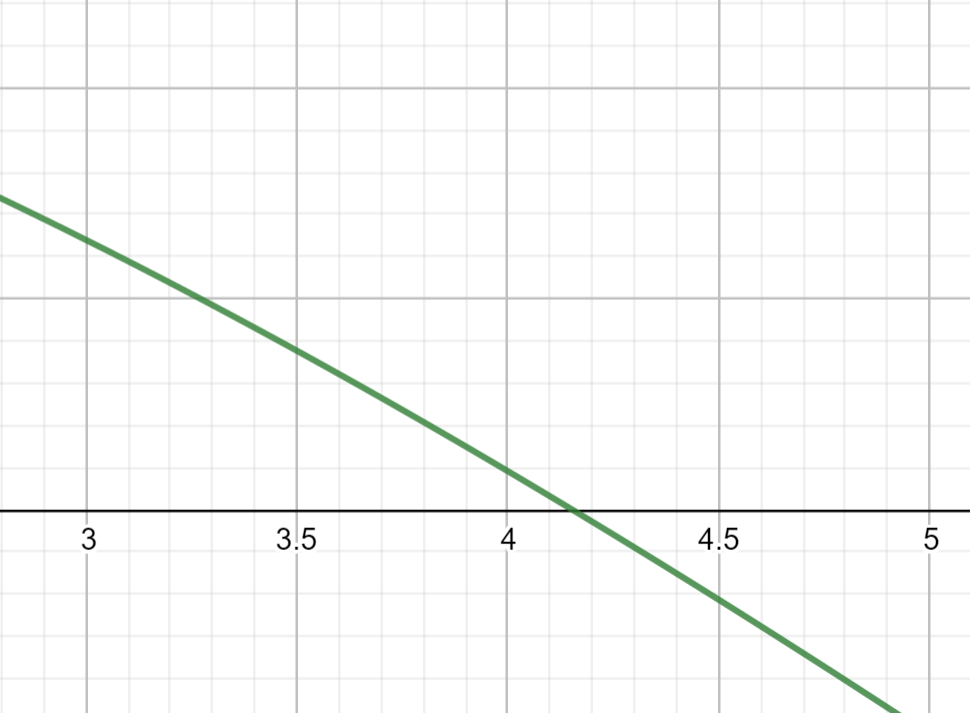
\includegraphics[width=8cm]{steffensen}
\end{center}
Si despejamos $x$ en la función y la llevamos a la forma $x=g(x)$ de la siguiente manera:
$$g(x)=ln(x^2 + x + 2)+1$$
Tomando el punto de partida $p_0=1$ y utilizando una tolerancia de 0.0005 obtenemos la siguiente tabla:
\begin{table}[h]
\begin{tabular}{|c|c|c|c|c|c|}
\hline 
Iteración & $p_i$ & $p_{i+1}$ & $p_{i+2}$ & $\widehat{p}_i$ & Error \\
\hline 
0 & 1 & 2.38629436111 & 3.31062222247 & 5.160068006305 & 4.160068006305\\
1 & 5.160068006305 & 4.52005746186 & 4.29401954606 & 4.17059800597 & 0.989470000327\\
2 & 4.17059800597 & 4.1597407368 & 4.15543254306 & 4.15259847380 & 0.017999532\\
3 & 4.15259847380 & 4.15259381389 & 4.15259196058 & 4.15259073675 & 7.7370422$\times 10^{-6}$\\
\hline 
\end{tabular} 
\end{table}
\subsubsection*{Procedimiento}
\begin{itemize}
\item \textbf{Iteracion:} 0 
	$$p_0=1 \hspace{1cm} p_1=g(p_0)=2.38629436111 \hspace{1cm} p_2=g(p_1)=5.160068006305$$
	Reemplazando en el acelerador de Aitken:
	$$\widehat{p}_0=1 - \dfrac{(2.38629436111 -1)^2}{5.160068006305-2\cdot2.38629436111+1}=5.160068006305$$
\item \textbf{Iteracion:} 1
	$$p_3=5.160068006305 \hspace{1cm} p_4=g(p_3)=4.52005746186 \hspace{1cm} p_5=g(p_4)=4.29401954606$$
	$$\widehat{p}_5=5.160068006305 - \dfrac{(.5200574618611 -5.160068006305)^2}{4.29401954606-2\cdot4.52005746186+5.160068006305}=4.17059800597$$
\item \textbf{Iteracion:} 2
	$$p_6=4.17059800597 \hspace{1cm} p_7=g(p_6)=4.1597407368 \hspace{1cm} p_8=g(p_7)=4.15543254306$$
	$$\widehat{p}_5=4.17059800597 - \dfrac{(4.1597407368  -4.170598005975)^2}{4.15543254306-2\cdot4.1597407368 +4.17059800597}=4.15259847380$$
\item \textbf{Iteracion:} 3
	$$p_9=4.15259847380 \hspace{1cm} p_{10}=g(p_9)=4.15259381389  \hspace{1cm} p_{11}=g(p_{10})=4.15259196058$$
	$$\widehat{p}_5=5.160068006305 - \dfrac{(4.15259196058 -4.15259847380)^2}{4.15259196058-2\cdot4.15259381389+4.15259847380}=4.15259073675$$
\end{itemize}
Si este ejercicio hubieramos realizado por el método de Punto Fijo, tendriamos 11 iteraciones. Y es por esto que el método de Steffensen resulta util.
\section*{Conclusión}
Hemos mostrado  las bases del Método de Steffensen, proveyendo una explicación de este algoritmo iterativo y los métodos que lo componen, proveyendo ejemplos.
\begin{thebibliography}{9}
\bibitem{LSCP} 
Shirley B. Pomeranz, \textit{Aitken's $\Delta^2$ method Extended}, University of York, UK, 2017. 
\bibitem{collomb}
Cedrick Collomb, \textit{A tutorial on the Aitken convergence accelerator}, nf. 
\bibitem{is}
Jaiswal J. P. \textit{Numerical Test}, University of Princeton, nf.
\bibitem{mm}
Patricia M. Fernandez, Graciela Molina, Leonardo Albarracin, \textit{Métodos NUmericos}, FACET-UNT, 2017.
\end{thebibliography}


\end{document}